% !TEX root = main.tex

\ \\[-1.0cm]
\subsection{Overview}\ \\[-0.7cm]
\label{eval}

\paragraph{Experiments} We conducted 3 groups of experiments: In the first group, we compare AMIE to two popular, state-of-the-art systems that are publicly available, WARMR~\cite{DehToi99,DehToi00} and ALEPH$^{\ref{foot:aleph}}$. 
In the second group of experiments, we compare the standard confidence to the novel PCA confidence that we have introduced in this paper (Section \ref{sec:model}).
In the third group of experiments, we run AMIE on different datasets to show the applicability of the system.

\paragraph{Settings} By default, AMIE finds all rules whose head coverage exceeds the default threshold of $\theta=1\%$. AMIE ranks the resulting rules by decreasing PCA confidence. There is no need to deviate from this default configuration when a user runs AMIE. There are no parameters to tune. All experiments with AMIE on all datasets are run in this setting, unless otherwise mentioned. 
% \comment{Katja}{Do have more details somewhere on why $\theta$ does not have to be tuned and its influence?}
% Fabian: no.

For some experiments, we want to compare AMIE's runtime with other systems. To have an equal basis, we make AMIE simulate the metrics of the competitor systems. AMIE can threshold on support, head coverage, confidence, and PCA confidence, and she can rank by any of these. AMIE can also count the support not on two variables, but on a single variable. AMIE can also output non-closed rules. Since this is just a choice of what to output, it does not influence runtime.
All experiments with all systems are run on a server with 48GB RAM and 8 CPUs. We always mine rules without constants (i.e., without the instantiation operator), unless otherwise mentioned. 

\paragraph{Knowledge Bases} We run our experiments on different KBs. In all cases, we removed the \emph{rdf:type} relationship, because it inflates the size of the KBs. We are aware that the \emph{rdf:type} relationship can be very helpful for rule mining. However, currently no approach (including ours) makes specific use of it. We plan to make use of it in future work. Furthermore, we removed all facts with literals (numbers and strings) from the KBs. Literal values (such as geographical coordinates) are shared by only very few entities, which makes them less interesting for rule mining.

\paragraph{Evaluations} In all experiments, our goal is twofold: First, we want to produce as many predictions as possible beyond the current KB. 
Second, the percentage of correct predictions shall be as large as possible.
The particular challenge is that we want to evaluate \emph{predictions that go beyond the current KB}. We are not interested in describing the existing data, but in generating new data.
Therefore, we proceed as follows: We run the systems on an older dataset (YAGO2~\cite{yago2}). We generate all predictions, i.e., the head atoms of the instantiated rules (see Section~\ref{sec:preliminaries}). We remove all predictions that are in the old KB.
Then we compare the remaining predicted facts to the successor of that dataset (YAGO2s \cite{yago2s}). A prediction is ``correct'' if it appears in the newer KB. A prediction is ``incorrect'' if it has a highly functional or highly inverse functional relation and contradicts an existing fact in the newer KB, e.g., a different birth place.
For all other predictions, we manually validated the facts by checking a sample of 30 of them against Wikipedia pages. This classifies the remaining predictions as ``correct'' or ``incorrect'' -- except for a few cases where the fact is ``unknown'', such as the death place of a person that is still alive. The ratio of correct predictions out of the correct and incorrect predictions yields the \emph{precision} of the rule.

\paragraph{Outlook} We note that with the project of predicting beyond current knowledge, we are entering a new, and very risky area of research. We do not expect Horn rules to have extraordinary precisions in the unknown region. Rules can only yield hypotheses about possible facts. 

\subsection{AMIE vs. WARMR and ALEPH}
\noindent In this section, we compare AMIE to WARMR and ALEPH. For each system, we conduct 3 experiments: We first compare the usability of the competitor system to AMIE. Then, we compare their runtimes. Last, we compare their outputs.%\\[-0.8cm] 

\subsubsection{AMIE vs. WARMR}

\paragraph{Usability} WARMR is a system that unifies ILP and association rule mining. Similar to APRIORI algorithms~\cite{Agrawal:1996:FDA:257938.257975}, it performs a 
%general to specific, 
breadth-first search in order to find frequent patterns.
% The difference to the traditional association rule mining systems (and the connection to ILP) is that WARMR does not add binary attributes on each level, but predicate calculus literals.
% These can form Datalog queries of the form
WARMR generates Datalog queries of the form ``$?-A_1,A_2,...,A_n$'',
where $A_i$ are logical atoms.

To discover frequent patterns (as in association rule mining), we need to have a notion of frequency. Given that WARMR considers queries as patterns and that queries can have variables, it is not immediately obvious what the frequency of a given query is. Therefore, the user needs to specify 
%define what is actually 
the predicate that is being counted by the system (the \textit{key predicate}). In the usual scenario of market basket analysis, e.g., the system counts customer transactions. In a scenario in which the database is a KB, one solution is to count entities. Since the key predicate determines what is counted, it is necessary that it is contained in all queries. Therefore, we add a predicate \emph{entity}$(x)$, which we fill with all entities of the KB. AMIE does not require such a choice. 


% WARMR requires the user to define the frequency of its queries. \comment{Katja}{More explanation necessary about what a query is.} Given that WARMR considers queries as patterns and that queries can have variables, it is not immediately obvious what the frequency of a given query is. Therefore, the user needs to define what is actually the predicate that is being counted by the system (\textit{key predicate}). \comment{Katja}{Jumps too fast into details. Difficult to grasp for the reader why we are talking all of a sudden about a predicate that is being counted and for what reason} In the usual scenario of market basket analysis, for example, the system counts customer transactions. In a scenario, in which the database is actually an ontology, one solution is to count entities. Since the key predicate determines what is actually counted, it is necessary that it is contained in all queries. Therefore, we add a predicate \emph{entity}$(x)$, which we fill with all entities of the KB. AMIE does not require such a choice.
% \comment{Katja}{I am not sure whether anyone without detailed knowledge about the topic would be able to understand the need for a key predicate and what the queries are that this paragraph is talking about.}

% The input for WARMR consists of files containing the facts in the database and the background knowledge. \comment{Katja}{Why all of a sudden distinguish between the data and the background knowledge? What is the background knowledge?}The user also needs to provide the language bias, i.e. to provide WARMR with specific information about which predicates are allowed to be added in a query, which of their variables could be new and which should have appeared in previously used literals (mode declarations), which arguments of predicates are allowed to be unified (type declarations). In contrast, AMIE requires none of these. AMIE simply takes as input the KB in triple format.

For WARMR, 
%The input for WARMR consists of files containing the facts and other necessary information. The 
the user needs to provide 
%the language bias, i.e. to provide WARMR with 
specific information about which predicates can be added to a query, which of their variables can be fresh, and which arguments of predicates are allowed to be unified (type declarations). In contrast, AMIE requires none of these. 
% \comment{actually AMIE also has a language bias targeted for rdf KBs. It is just that the user cannot change the bias}.
% Fabian: yes. let's not emphasize it here...
AMIE simply takes as input the KB in triple format.

WARMR is also able to mine rules with constants. The user can define which predicates and arguments should be instantiated with constants (we call this mode MODE1). WARMR then checks all the constants appearing in the facts of that specific predicate and argument and afterwards uses them in the queries. 
MODE1 naturally entails an increase of the branching factor in the search space and an explosion in the number of candidates that need to be evaluated. Alternatively, WARMR allows the user to set a maximum number of constants to be used for each predicate and argument (MODE2). Unfortunately, though, it does not provide a way for the user to influence the selection of these constants. In other words, there is no guarantee that the constants that WARMR will use are the most promising ones. 

WARMR produces rules as output. These rules are not necessarily connected. For example, WARMR mines
\indented{\emph{isMarriedTo}(B,C),  $\wedge$ \emph{isLeaderOf}(A,D)\\ $\Rightarrow$ \emph{hasAcademicAdvisor}(C,E)}
This rule is not only nonsensical from a semantic perspective, but also redundant, because the second atom does not influence the implication. Therefore, the user has to filter out these rules from the output.

Thus, we conclude that the broader mission and the broader applicability of WARMR entails that much more configuration, acquaintance, and expert knowledge is needed to make it mine Horn rules on semantic KBs.
%\comment{Katja}{Do we have a good justification in the paper why Horn rules are enough?}
%\comment{chris}{I don't think so. Actually they are not necessarily enough. This is why there is so much related work on the DL side}

\paragraph{Runtime} 
% \ignore{We wanted to ran AMIE and WARMR on the YAGO2s\cite{yago2s} dataset. YAGO2s contains around 4 million facts about 1.6 million entities. WARMR counts support on the key predicate, which contains one variable. Therefore, we also had AMIE count support on one variable. WARMR thresholds on support. Therefore, we also made AMIE threshold on support. We ran both systems with a support threshold of 80,000 (5\% of the total number of entities). 
% AMIE completed her task on this dataset in \comment{?}{minutes}. }
% YAGO2s\cite{yago2s} contains around 4 million facts about 1.6 million entities. WARMR was not able to operate on this dataset: It aborted due to the size of the data. We could not make it run on YAGO2s, also after checking back with the WARMR team. 
% Therefore, we created a sample of YAGO2s. Randomly selecting a number of facts from the initial dataset could break the interesting links between the entities. Therefore, we randomly selected 10,000 seed entities and included their 3-hop neighborhood. This yielded 48k entities and 79k facts. This sample contains all available information in a radius of 3 hops around the seed entities, but much less information about the entities at the periphery of the subgraph. Therefore, we restricted the values for the key predicate
% %(used to assign frequencies to the rules)
% to seed entities only. 
YAGO2\cite{yago2} contains around 940K facts about 470K entities. 
WARMR was not able to terminate on this data in a time period of 1 day. Therefore, we created a sample of YAGO2. 
Randomly selecting a number of facts from the initial dataset could break the interesting links between the entities. 
Therefore, we randomly selected 10,000 seed entities and included their 3-hop neighborhood. 
This yielded 14K entities and 47K facts. 
This sample contains all available information in a radius of 3 hops around the seed entities, but much less information about the entities at the periphery of the subgraph. 
Therefore, we restricted the values for the key predicate
%(used to assign frequencies to the rules)
to the seed entities only. 

% Since the sample is much smaller than the original KB, we lowered the support threshold to 5 entities. We ran AMIE with these parameters on the sample. AMIE mined her rules in 29.43 seconds.
% WARMR, in contrast, 
% took 19.2 hours. We also ran both systems allowing them to mine rules with constants. AMIE completed the task in 21 minutes. WARMR in MODE1 did not terminate in 3 days. Therefore, we ran WARMR in MODE2.
% To have reasonable runtimes, we allowed WARMR to find constants only for one predicate (\emph{diedIn}). We also restricted it to find only 20 constants. WARMR ran in 19.7 hours. Table \ref{warmrruntime} summarizes the runtime results. We conclude that AMIE is better suited for large KBs than WARMR. This is because WARMR is an ILP algorithm written within a logic programming environment, which makes the evaluation of all candidate queries inefficient.

Since the sample is much smaller than the original KB, we lowered the support threshold to 5 entities. We ran AMIE with these parameters on the sample. AMIE mined her rules in 3.90 seconds.
WARMR, in contrast, took 18 hours. 
We also ran both systems allowing them to mine rules with constants. AMIE completed the task in 1.53 minutes. WARMR in MODE1 for all relations did not terminate in 3 days. 
Therefore, we ran it also only for the relations \textit{diedIn}, \textit{livesIn}, \textit{wasBornIn}, for which it took 48h. We also ran WARMR in MODE2.
To have reasonable runtimes, we allowed WARMR to find constants only for one predicate (\emph{diedIn}). We also restricted it to find only 20 constants. WARMR ran 19 hours. 
Table \ref{warmrruntime} summarizes the runtime results. We conclude that AMIE is better suited for large KBs than WARMR. 
This is because WARMR is an ILP algorithm written in a logic programming environment, which makes the evaluation of all candidate queries inefficient.\\

\ffigure{Table}{warmrruntime}{Runtimes on YAGO2 Sample}{
\footnotesize
\begin{tabular}{l|rr}
Constants & WARMR & AMIE\\
\hline
 no & 18h & 3.90s\\
 yes & (48h) / (19.3h) & 1.53min \\
\end{tabular}
}

\paragraph{Results} After filtering out non-connected rules, WARMR mined 41 closed rules. AMIE, in contrast, mined 207 closed rules, which included the ones mined by WARMR. 
We checked back with the WARMR team and learned that for a given set of atoms $B_1, ... B_n$, WARMR will mine only one rule, picking one of the atoms as head atom (e.g., $B_1 \wedge ... \wedge B_{n-1} \Rightarrow B_n$). AMIE, in contrast, will mine one rule for each possible choice of head atom (as long as the thresholds are met). In other words, AMIE with the standard support and confidence measures simulates WARMR, but mines more rules. Furthermore, it runs orders of magnitude faster. Especially for large datasets for which the user would have needed to use complicated sampling schemes in order to use WARMR, AMIE can be a very attractive alternative. Even for smaller datasets with rules with constants, AMIE can provide results while WARMR cannot. Moreover, AMIE comes with metrics that go beyond the standard confidence and the standard support. We will show later that these improve the quality of the results.

\subsubsection{AMIE vs. ALEPH}

\paragraph{Usability} ALEPH can be run with different commands that influence the search strategy. We chose the \emph{induce} command, which runs fastest. 
For running ALEPH, the user has to specify the target predicate for learning (the head predicate of the rules). 
In the following, we ran ALEPH successively with all predicates of the KB as targets. 
In addition, the user has to specify a series of type and mode declarations (similar to WARMR), which will be used as a language bias in order to restrict the search space. 
In addition, the user needs to provide ALEPH with files containing the background knowledge and positive examples for the target predicate. 
In contrast, AMIE requires no such input. It will run on a KB without any prespecified choices of predicates.\\

\ffigure{Table}{alephrun0}{Runtimes ALEPH vs. AMIE}{
\footnotesize
\begin{tabular}{l|l|cc}
KB & Facts & ALEPH & AMIE\\
\hline
YAGO2 full & 948k & 4.96s to $>$ 1 day & 3.62min\\
YAGO2 Sample & 47k & 0.05s to $>$ 1 day & 5.41s\\
\end{tabular}
}%\ \\[-1cm]

\ffigure{Table}{alephrun1}{Runtimes of ALEPH on YAGO2}{ % no constants
%\begin{flushleft}
\begin{tabular}{l|r}
Relations & Runtime\\
\hline
isPoliticianOf, hasCapital, hasCurrency & $<$ 5min\\
dealsWith, hasOfficialLanguage, imports & $<$ 5min\\
isInterested, hasMusicalRole & $<$19min\\
hasAcademicAdvisor, hasChild& $>$ 1 day\\
isMarriedTo, livesIn, worksAt, isLocatedIn& $>$ 1 day\\ %[-0.4cm]
\end{tabular}
%\end{flushleft}
} %\ \\[-1cm]

\ffigure{Table}{alephrun2}{Runtimes of ALEPH on YAGO2 Sample}{
%\begin{flushleft}
\begin{tabular}{l|r}
Relations & Runtime\\
\hline
diedIn, directed, hasAcademicAdvisor & $<$ 2min\\
graduatedFrom, isPoliticianOf, playsFor & $<$ 2min\\
wasBornIn, worksAt, isLeaderOf &  $<$ 2min\\
exports, livesIn, isCitizenOf & $<$ 1.4h\\
actedIn, produced, hasChild, isMarriedTo & $>$ 1 day\\ %[-0.4cm]
\end{tabular}
%\end{flushleft}
}%\ \\[-1cm]

\paragraph{Runtime} 
% We ran AMIE and ALEPH on YAGO2 \cite{yago2}. For ALEPH, we used the positive-only evaluation function with $Rsize=50$ and we considered only clauses that were able to explain at least 100 positive examples. 
% %Since ALEPH thresholds on support, we also instructed AMIE to threshold on support, and we chose the same threshold value of 100.
% In order to guarantee fair comparison, we also instructed AMIE to run with a support threshold of 100 facts.
% AMIE terminated in 4.5 minutes, and found rules for all relations. ALEPH ran for one head relation at a time. For one relation (\emph{isPoliticianOf}), it terminated in a few seconds. 
% For others, however, we had to abort the system after one day without results (Tables \ref{alephrun0} and \ref{alephrun1}). 
% For each relation, ALEPH treats one positive example at a time. Some examples need little processing time, others block the system for hours. 
% We could not figure out a way to choose examples in such a way that ALEPH runs faster. 
% Hence, we created a sample of YAGO2 as for WARMR, containing around 170,000 facts for a variety of target predicates. 
% We decreased the support threshold to 2. Again, runtimes varied widely between relations (Table \ref{alephrun2}). 
% Some relations ran in a few seconds, others did not terminate in a day. 
% The runtimes with constants are similarly heterogenous, with at least 4 relations not terminating in 3 days.\\
We ran AMIE and ALEPH on YAGO2 \cite{yago2}. For ALEPH, we used the positive-only evaluation function with $Rsize=50$ and we considered only clauses that were able to explain at least 2 positive examples, 
so that we will not get grounded facts as rules in the output. 
For a fair comparison, we also instructed AMIE to run with a support threshold of 2 facts.
AMIE terminated in 3.62 minutes, and found rules for all relations. ALEPH ran for one head relation at a time. For some relations (e.g.\emph{isPoliticianOf}), it terminated in a few seconds. 
For others, however, we had to abort the system after 1 day without results (Tables \ref{alephrun0} and \ref{alephrun1}). 
For each relation, ALEPH treats one positive example at a time. Some examples need little processing time, others block the system for hours. 
We could not figure out a way to choose examples in such a way that ALEPH runs faster. 
Hence, we used the sample of YAGO2 that we created for WARMR.
%, which contains around 47k facts for a variety of target predicates. 
Again, runtimes varied widely between relations (Table \ref{alephrun2}). 
Some relations ran in a few seconds, others did not terminate in a day. 
The runtimes with constants are similarly heterogenous, with at least 7 relations not terminating in 1 day.

\paragraph{Results} 
% We compared the output of ALEPH on the head relations for which it terminated to the output of AMIE on these head relations. 
% ALEPH mined 15 rules, while AMIE mined 306 rules. Table \ref{alephres} shows the number of predictions, and their total precision as described in Section \ref{eval}. 
% We show the aggregated values for the top 11 rules (at which point both approaches produce roughly the same number of predictions), 
% for the top 15 rules (which is the number of rules ALPH produced) and for the top 30 rules for AMIE. AMIE produces predictions of a much better quality than ALEPH. 
% We suspect that this is because ALEPH's positives-only evaluation function manages to filter out overly general rules only to some extend. 
% ALEPH will mine, e.g, \emph{livesIn}$(A,B) \Rightarrow$ \emph{isPoliticianOf}$(A,B)$.
% %Table~\ref{tblAleph} shows examples of overly general rules that ALEPH produces. Consider the third rule: this rule will infer for every person that lives somewhere that this person is also a politician of that place, which is obviously wrong.
% The problem is that ALEPH generates counterexamples by randomly using valid constants for variables $A$ and $B$. 
% This means that the probability of creating a random example in which $B$ is the place of residence of the specific person $A$ is very low. 
% AMIE's rules, in contrast, produce many predictions, and also have a much better precision in the unknown region. 
% All rules output by both systems are available online at \url{http://www.mpi-inf.mpg.de/departments/ontologies/projects/amie/}.\\
We compared the output of ALEPH on the head relations for which it terminated to the output of AMIE on these head relations, on the sample dataset. 
ALEPH mined 56 rules, while AMIE mined 335 rules. We order the rules by decreasing score (ALEPH) and decreasing PCA confidence (AMIE). Table \ref{alephres} shows the number of predictions, and their total precision as described in Section \ref{eval}. 
We show the aggregated values at the points where both approaches have produced around 3K, 5K and 8K predictions.
AMIE's PCA confidence succeeds in sorting the rules roughly by descending precision, so that the initial rules have an extraordinary precision compared to ALEPH's. AMIE needs more rules to produce the same number of predictions as ALEPH (but she also mines more).
We suspect that ALEPH's positives-only evaluation function manages to filter out overly general rules only to some extent. 
ALEPH will mine, e.g, \emph{livesIn}$(A,C),$\emph{isLocatedIn}$(C,B) \Rightarrow$ \emph{isPoliticianOf}$(A,B)$.
%Table~\ref{tblAleph} shows examples of overly general rules that ALEPH produces. Consider the third rule: this rule will infer for every person that lives somewhere that this person is also a politician of that place, which is obviously wrong.
The problem is that ALEPH generates counterexamples by randomly using valid constants for variables $A$ and $B$. 
This means that the probability of creating a random example in which $B$ is the place of residence of the specific person $A$ is very low.\\ 

\ffigure{Table}{alephres}{Top Rules of ALEPH vs. AMIE}{
\begin{tabular}{l|rrr}
 System & Top $n$ & Predictions & Precision \\
 \hline
 ALEPH & 7 & 2997 & 27\% \\
 AMIE & 13 & 3180 & 66\% \\
 \hline
 ALEPH & 9 & 5031 & 26\% \\
 AMIE & 29 & 5003& 47\% \\
 \hline
 ALEPH & 17 & 8457 & 30\% \\ 
 AMIE & 52 & 8686  & 45\% \\
\end{tabular}
}

\ignore{
\begin{table*}\label{tblAleph}
\begin{center}
% use packages: array
\begin{tabular}{lc}
\textbf{Rule} 							& \textbf{Learned by AMIE}\\
isPoliticianOf(A,B) :- wasBornIn(A,C), isLocatedIn(C,B) 	&  	\\ 
isPoliticianOf(A,B) :- diedIn(A,C), isLocatedIn(C,B)		&  	\\ 
isPoliticianOf(A,B) :- livesIn(A,B) 				&  	\\
directed(A,B) :- created(A,B)					&	\\
directed(A,B) :- produced(A,B)					&	\\
isLeaderOf(A,B) :- livesIn(A,B).				&	\\

\end{tabular}
\end{center}
\caption{Examples of overly general rules learned by ALEPH}
\end{table*}
}

\subsection{AMIE with Different Metrics}

In this section, we compare the standard confidence measure to the PCA confidence measure. 
We ran AMIE with the default head coverage threshold on the YAGO2 dataset. It contains nearly 500K entities and 948K facts. 
We sort the rules first by descending PCA confidence, and then by descending standard confidence, and look at the top rules.
For each rule, we evaluated the predictions beyond YAGO2 as described in Section \ref{eval}. 
Figure \ref{finalshow} uses aggregated predictions and aggregated precision to illustrate the results. 
The $n$-th dot from the left tells us the total number of predictions and the total precision of these predictions, aggregated over the first $n$ rules.
As we see, ranking the rules by standard confidence is a very conservative approach: 
It identifies rules with reasonable precision, but these do not produce many predictions. 
Going down in the list of ranked rules, the rules produce more predictions -- but at lower precision. The top 30 rules produce 113K predictions at an aggregated precision of 32\%.
If we rank the rules by PCA confidence, in contrast, we quickly get large numbers of predictions. The top 10 rules already produce 135K predictions -- at a precision of 39\%.
The top 30 rules produce 3 times more predictions than the top 30 rules by standard confidence -- at comparable precision.
This is because the PCA confidence is less conservative than the standard confidence. 
%At the same time, the precision of the resulting rules is higher. 
%Even as we go lower in the ranked list, the precision remains higher.


\ffigure{Figure}{finalshow}{Std. Confidence vs. PCA Confidence}{
\hspace*{-5ex}
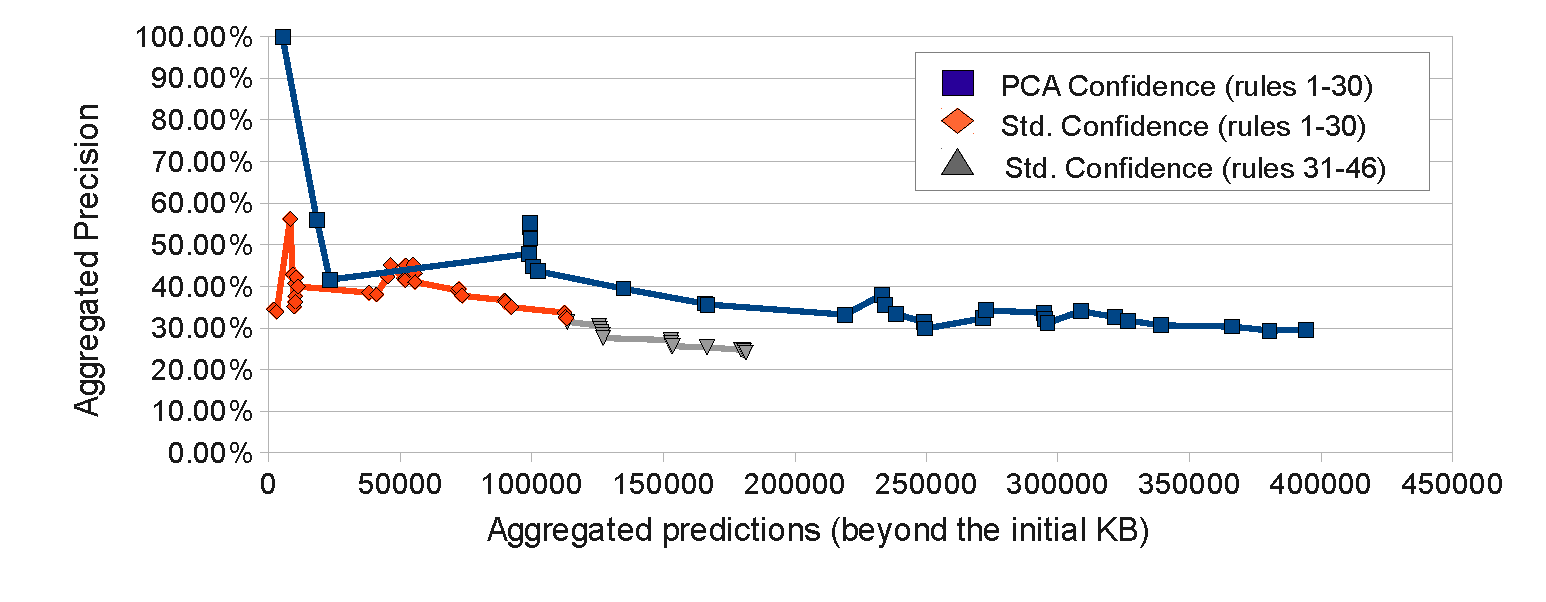
\includegraphics[scale=0.38]{figures/pca_vs_std_confidence.pdf}\ \\[-0.5cm]
}

\paragraph{Discussion} The precision of the rules is in the range of 30\%-40\%. 
Thus, only a third of the predictions in the unknown region will be correct. Still, even imperfect rules can be useful: 
If, e.g., a human checks the facts before they are added, then reducing the number of false predictions is a great advantage. 
If games with a purpose are employed, then the rules can help pre-select candidate facts. If multiple sources are combined, then rules can contribute evidence. 
If reasoning approaches are used, then rules can be taken into consideration according to their estimated performance. Finally, the precision is better if 
standard confidence is used. %Finally, the precision of the PCA confidence is better than if standard confidence is used.

\paragraph{Predicting Precision} 
%Another advantage of the PCA confidence is that it estimates the precision of the new facts better than the standard confidence. 
%If we consider the precision of a rule as the probability for its predictions to be true, and the standard and PCA confidence as estimates for such probability, 
%we can calculate the average error of these estimates over all produced facts. 
The confidence measures can serve to estimate the actual precision of a rule.
In Table  \ref{cor}, we rank the mined rules by their precision and report the average absolute error of the standard and PCA confidence weighted by the number
of predictions produced by the rules. We can observe that, on average, the PCA confidence estimates the precision of the rules better than the normal confidence. 
Thus, reasoning approaches can use the PCA confidence as a weight for the rule.\\
%It is also important to remark, that the PCA confidence achieves a reduction up to 57\% (top 20 rules) in the error with respect to the standard confidence. 
%Since the error of PCA confidence is much smaller than the error of the standard confidence for the best performing rules (in terms of the actual precision), our results also imply that
%such rules have higher chance to be discovered during the mining process, if we use the PCA confidence for ranking or output pruning.\\

\ffigure{Table}{cor}{Average Absolute Error to Precision}{
\begin{tabular}{l|ccc}
		& Top 20 rules 	&Top 30 rules	&All rules	\\
\hline
Confidence 	& 0.76		&0.63		&0.33 \\
PCA Confidence 	& 0.32		&0.29		&0.29 \\
\end{tabular}
}



We also note that our rules are insightful. Table \ref{rules} shows some of the rules we mined. Being able to mine reasonable rules on semantic KBs of this size is an achievement beyond the current state of the art.\\

\ffigure{Table}{rules}{Some Rules by AMIE}{
\begin{tabular}{|l|}
\hline
\emph{isMarriedTo}$(x,y) \wedge$ \emph{livesIn}$(x,z) \Rightarrow $ \emph{livesIn}$(y,z)$\\
\emph{isCitizenOf}$(x,y) \Rightarrow$ \emph{livesIn}$(x,y)$\\
\emph{hasAdvisor}$(x,y) \wedge $ \emph{graduatedFrom}$(x,z) \Rightarrow$ \emph{worksAt}$(y,z)$\\
\emph{wasBornIn}$(x,y) \wedge$ \emph{isLocatedIn}$(y,z) \Rightarrow$ \emph{isCitizenOf}$(x,z)$\\
\emph{hasWonPrize}$(x,G.\;W.\;Leibniz) \Rightarrow$ \emph{livesIn}$(x,Germany)$\\
\emph{hasWonPrize}$(x,Grammy) \Rightarrow$ \emph{hasMusicalRole}$(x,Guitar)$\\
\hline
\end{tabular}
}

\subsection{AMIE on Different Datasets}
As a proof of concept, we ran AMIE on YAGO2 \cite{yago2}, YAGO2 with constants, and DBpedia \cite{dbpedia}. We chose an older version of DBpedia (2.0), so that we can evaluate the output to a newer version of DBpedia (3.8). 
Due to the large number of relations in DBpedia 2.0, there is an enormous number of rules to be found. We show the time taken to mine rules with 2 atoms. 
We provide also the number of predicted facts that are in the newer version of the KB but not in the old one (hits). As Table \ref{dbp} shows, AMIE can produce rules with or without constants in a reasonable time.\\

 \ffigure{Table}{dbp}{AMIE on Different Datasets}{
 \small
 \begin{tabular}{l|rr|rrr}
 Dataset & Entities & Facts & Runtime & Rules & Hits \\
 \hline
 YAGO2   &  470475 &  948044  & 3.62min &  138   &  74K \\
 YAGO2 const  &    470475    &  948044  &  17.76min  &  18886   & 159K \\
 DBpedia &  1376877   & 6704524  &    2.89min  &  6963    &  122K \\
 \end{tabular}
 }

 \noindent All rules and all experimental results are available at \url{http://www.mpi-inf.mpg.de/departments/ontologies/projects/amie/}.